\chapter{\fontsize{15}{12}\selectfont Implementations of machine learning algorithms}

\section{Random Forest}
\subsection{Data Preparation}
In addition to all of the data manipulation and preparation we did to our datasets, we need, in fact, one last preparation phase in order to correctly train the model with our data. 

Since we work with a regressor random forest (and not a classifier), the model requires numerical data, which mean, for instance, the home\_team and away\_team features (=columns) need to be modified into numerical values.
To achieve this, we one-hot encoded all our categorical features.
One-hot encoding in machine learning is the conversion of categorical information into a format that may be fed into machine learning algorithms to improve prediction accuracy.


To achieve this, we one-hot encoded all our categorical features.
One-hot encoding in machine learning is the conversion of categorical information into a format that may be fed into machine learning algorithms to improve prediction accuracy.

What it does in practice is to "divide" a feature into n features, where n is the amount of distinct values the feature had.

For example, the following dataframe:
\begin{table}[h]
  \centering
  \begin{tabular}{|c|}
    \hline
    Country\\
    \hline
    France
     \\
    \hline
    England\\
    \hline
    Wales\\
    \hline
  \end{tabular}
  \label{tab:exemple}
\end{table}


Will be encoded into the following dataframe:\\
\begin{table}[h]
  \centering
  \begin{tabular}{|c|c|c|}
    \hline
    Country\_France & Country\_England & Country\_Wales \\
    \hline
    1 & 0 & 0 \\
    \hline
    0 & 1 & 0 \\
    \hline
    0 & 0 & 1 \\
    \hline
  \end{tabular}
  \label{tab:exemple}
\end{table}

\newpage
Using that method, we encoded every categorical features of our final dataset. 
One other preparation we could have done for the model is to normalize our numerical values, to ensure every feature has the same impact and "weight"
However, in the case of Random Forests, the nature of the algorithm, which builds decision trees based on feature splits, inherently handles varying scales without the need for explicit normalization.

We tested this property and found it was true.\\
\begin{figure}[h]
  \centering
  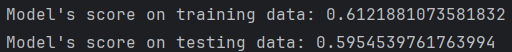
\includegraphics[width=0.8\linewidth]{withNormalization.png}
  \caption{Model's accuracy with the normalization}
\end{figure}

\begin{figure}[h]
  \centering
  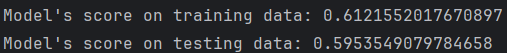
\includegraphics[width=0.8\linewidth]{withoutNormalization.png}
  \caption{Model's accuracy without the normalization}
\end{figure}

\subsection{Training and best parameters}
Our data is finally ready to be used by the random forest regressor.
As mentionned earlier, we used scikit learn's RandomForestRegressor class as our model.
The regressor variant allows us to target multiple features to predict in contrary to the classifier random forest.
We chose to predict the $home\_score$ and $away\_score$, the amount of goals the teams scored.
Scikitlearn also proposes the GridSearchCV class, a very powerful tool that will determine the best possible parameters configuration for the model.

Once created and set with the best parameters, we need to train the model with our dataset. 
It's our final step before being able to predict a match.

In order to train the model we must split our dataframe into the training samples and the testing samples.
We did that using the $test\_train\_split()$ function from scikitlearn model selection library.
We decided to take 70\% of the dataframe for training purpose and thus 30\% for testing.

For the training, scikitlearn proposes an already built-in function for the RandomForestRegressor class which is fit() that we used.
In fact, things are a bit different in the project because we train the GridSearchCV, and we extract our trained model from this object.

\begin{verbatim}
randomForestModel = RandomForestRegressor(random_state=1)
randomForestGridSearch = 
GridSearchCV(randomForestModel, params, cv=5, verbose=1, n_jobs=-1)
\end{verbatim}

\noindent Then we train the model
\begin{verbatim}
randomForestGridSearch.fit(X_train, y_train)
\end{verbatim}

\noindent We apply to our model the best parameters found by the grid search
\begin{verbatim}
randomForestModel = randomForestGridSearch.best_estimator_
\end{verbatim}


\subsection{Prediction}
To predict a match or a championship (see Championship part later) we need to give to our model an entry (a row) in the shape of what it has been trained on. Basically speaking, we give him as input a dataframe with a single row, without, obviously, the features to predict (the scores).
The input also needs to be encoded the exact same way the training set was.
In our code, the getMatchDataframe() does this job, with just the names of the playing countries and the city/country host of the match, we fetch all the remaining data to have our input.

For example we fetch the latest rank from the FIFA ranking dataset, the latest averageScore from $rera\_improved$ and so on ...
Also, the tournament in which the match takes place is always the FIFA World cup.
We also one hot encode the dataframe the same way it was done for the model training set

Finally, we use the predict() method of the model on that dataframe describing the match to predict the resulting scores.
We convert these scores into a probability of winning with an exponential fonction. The team with the highest probability wins. If the probabilites are near 50\%, we "simulate" a shootout. (See shoutouts part)

\subsection{Accuracy}
Our regressor random forest has an accuracy of near 60\% on the testing set, which is not very good.
Also, it appears that the model has a mean square error near 1, which is extremely high considering the predicted scores vary between 0.2 and 2.0.
Even although to us humans, the results are pretty decent, in a mathematical point of view the model is pretty unusable.
\subsection{Difficulties encountered for the Random Forest}
During the implementation of the Random Forest regressor, we met two main issues:
 \begin{itemize}
    \item[-] Understanding how to prepare the data for training the model was the hardest and longest part, which made us rollback 2 days of work to restart on a good base.
    \item[-] The most complex one: the model seems to very largely advantage the $home\_team$ even if the match is played at a neutral location.

\end{itemize}
	In others words, France - England would output France as the winner, and England - France would output England even if the matches were played in Australia for instance.
	Except when the strength difference was enough to outpower that disadvantage, the team on the left was always winning.
	To counter this bias we decided to predict two times the match, once A vs B and a second time B vs A. We then chose as the winner the winner of the match which had the biggest score difference, we thought it was a good solution.
\newpage
\section{Neural Network regressed}


\textbf{Variables Correlation}\\
\\
The correlation is a statistical metric that determines the relationship between two variables. If two variables are highly correlated then we can predict one from the other.therefore,we should provide to our model only features that are highly correlated with our target
for this purpose we used matplotlib library,the plt.show method displays the correlation between the columns of our dataset

\begin{figure}[h]
  \centering
  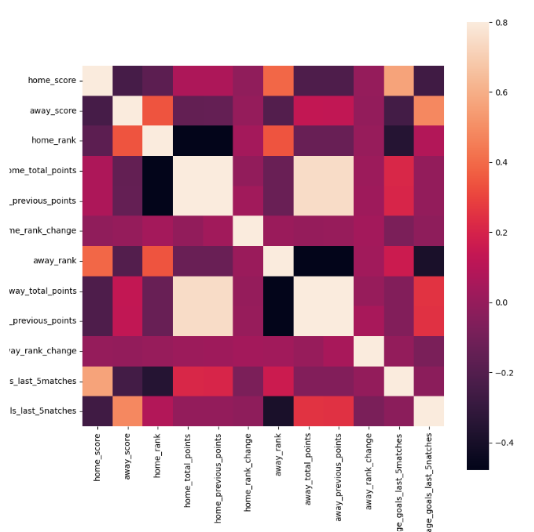
\includegraphics[width=0.8\linewidth]{NNLregressor.png}
  \caption{Correlation between columns}
\end{figure}
 
\noindent \textbf{Neural Network Regressor}\\
\\
After implementing any Machine learning Model,it is highly recommended to implement another model in order to be able to evaluate  its performance compared to other models,this also allows us to find out whether some particular models are better for predicting our dataset.
 In this section,we are going to implement a Neural Network Regressor and compare its performances to the Random forest model implemented in the previous section\\
\newpage

 \begin{quote}
\textbf{Data preparation}\\
\\
Since we have already prepared our data in the previous section for training the Random Forest Model we decided to use the same data for the Neural Network Regressor.\\
\\
\textbf{Implementation}\\
\\ 
We used scikit-learn which is a very popular library for python that provides various implementation of neural network regressors and we created an MLPRegressor using 3 parameters:\\
 \begin{quote}
hidden\_layer\_size: this parameter represents the number of neurons in each hidden layer,in our case we used 2 hidden layers with 100 neurons each\\
\end{quote}
 \begin{quote}
activation: we used the logistic sigmoid as the activation function for the hidden layers.\\
\end{quote}
 \begin{quote}
max\_iter: this parameter represents the maximum number of iterations for the solver to converge, we set it to 1000
After defining our model we call the fit method in order to train our model on the provided training data\\
\end{quote}
\end{quote}

\\
\noindent \textbf{Results}
\\
The neural network model is not giving very good results comparing to the random forest\\


\noindent \textbf{Conclusion}\\

\noindent We can conclude that the neural networks,especially deep learning models, require very huge amount of data in order to give good results and avoid overfitting,and since our dataset is tabular and small it is more recommended to use simpler models like decision trees or random forest .this conclusion leads as to say that the choice of the most performant algorithm depends on the specific problem and the structure of the dataset 


\newpage
\section{Championship}
One goal of this project was to predict a championship.
The championship is in the shape of a .csv file containing the team groups.\\

\noindent First comes the group phase, where each team in a group plays a match against every other country in the same group. A win results in obtaining 3 points, and a draw 1 point for both team, there are no shootouts in this phase.\\

\noindent Once all the matches are played, the two teams with the highest points of their team go to the knockout phase. 
The knockout phase, the looser is eliminated and the winner goes to the next match, until one team is left, the champion.
In this phase, if the model outputs a very similar probability of winning for both teams, we simulate a shootout between the two teams. (See shootouts part)\\

\noindent Example of a championship predicted by the regressor random forest -
Here we tried to predict the 2022 world cup
\begin{figure}[h]
  \centering
  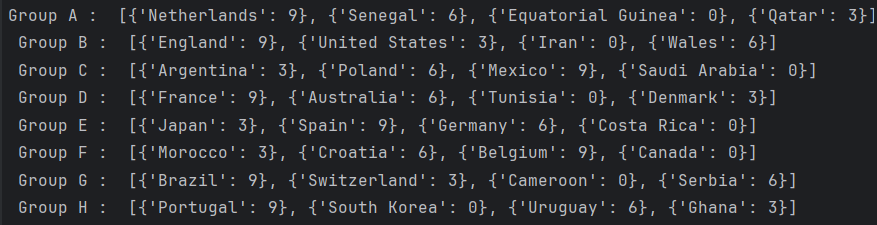
\includegraphics[width=0.8\linewidth]{cdmGroupPhase.png}
  \caption{Group phase results with each team points}
\end{figure}

We can observe two main "anomalies" in these results, the Argentina is eliminated without reaching the knockout phase, and the Mexico won all its matches.
It is very hard to predict a World Cup since pretty much everything can happen (see for example Morocco's performance in World cup 2022), so calling it an anomaly isn't very pertinent.

\begin{figure}[h]
  \centering
  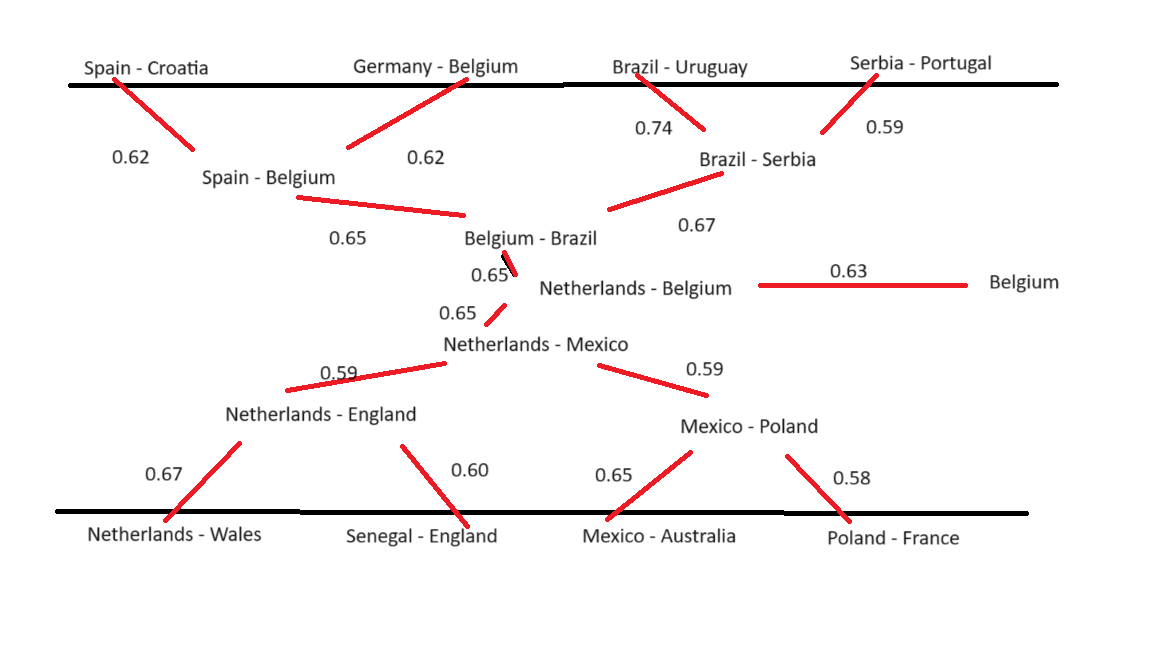
\includegraphics[width=0.8\linewidth]{championshipPaint.png}
  \caption{Knockout phase with the probabilities of win for every match}
\end{figure}

\newpage
\section{Shootouts}
To simulate the shootouts between two teams in the case of a draw (except during group phase), we decided not to use any machine learning technique: integrating the shootouts in the dataset the model learns from was almost impossible, and considering how extremely rare we face a draw with our models, creating another model, whose sole purpose would be to predict the outcome of the shootouts, was overkill and a loss of time.
To determine the winner of a shootouts, we simply check the history of shootouts between the two teams, if A has beaten B more times than B beat A, then A wins, if they are equals in terms of wins against eachother, the highest ranked team wins.
It is a very naive way of predicting the winner, creating another model to solely predict the shootouts would be the best option.
